\chapter{Transformations du plan et fonctions complexes}


\section{Introduction}

L'objectif du cours est l'étude des fonctions de la variable complexe  prenant leur valeurs dans le plan complexe. Plusieurs points de vue permettent d'appréhender ces fonctions, celui que nous privilégierons consistera à interpréter toute fonction $f$ comme une règle de transformation du plan complexe~; au point $z \in \C$ est associé le point $\omega=f(z)$ dans $\C$. Cette vision géométrique, outre le fait qu'elle offre une approche très visuelle de ces fonctions, est très importante de point de vue théorique. Elle dérive historiquement des problèmes de cartographie de la Terre qui furent étudiés par Gauss, Mercator, Lambert, Euler et Lagrange. Le problème consistait à représenter la sphère sur le plan en demandant par exemple~: la préservation des aires (carte équivalente), la préservation des angles (carte conforme), la préservation des distances (carte équidistante) ou enfin la préservation de certaines courbes privilégiées (carte orthodromique, carte loxodromique). Rappelons l'impossibilité d'appliquer homéomorphiquement la sphère sur le plan, la sphère étant compacte à la différence du plan. Contourner ce défaut nécessite de compactifier le plan en ajoutant un point à l'infini. L'espace ainsi obtenu est alors homéomorphe à la sphère, dite sphère de Riemann, et cet homéomorphisme est connu sous le nom de projection stéréographique. Nous verrons que pour étudier les transformations du plan, il est souvent plus simple de travailler sur la sphère de Riemann, car en particulier les droites du plan correspondent aux cercles passant par le pôle Nord de la sphère de Riemann, image du point à l'infini. Ainsi, aux transformations de la sphère de Riemann qui préservent les cercles correspondent les transformations du plan qui préservent la famille des cercles et des droites~; par exemple à une translation du plan transportant l'origine au point $P$ correspond la rotation de la sphère de Riemann transportant le pôle Sud en l'image du point $P$.   


%Une autre raison profonde de cette impossibilité, découverte par Gauss (à vérifier) provient du fait que la sphère à une courbure positive, matérialiser par le fait que la somme des angles inscrit dans une triangle tracé sur celle-ci est strictement supérieure à $\pi$, ceci à la différence du plan. 

%\begin{exer}
%Soit un triangle $T$ tracé sur une sphère de rayon $R$ en joignant trois points distincts par des arcs de grand cercle (qui correspondent aux droites du plan). En prolongeant les côtés du triangle, observer que la sphère est subdiviser en quatre triangles $T, T_\alpha, T_\beta, T_\gamma$, et en déduire que la somme des aires $\mathcal{A}$ des triangles vérifie l'identité
%$$\mathcal{A}(T) + \mathcal{A}(T_\alpha)+\mathcal{A}(T_\beta)+\mathcal{A}(T_\gamma)=4 \pi R^2.$$
%Ensuite vérifier visuellement les relations suivantes~:
%\begin{align*}
%\mathcal{A}(T)+\mathcal{A}(T_\alpha)&=2 \alpha R^2\\
%\mathcal{A}(T)+\mathcal{A}(T_\beta)&=2 \beta R^2\\
%\mathcal{A}(T)+\mathcal{A}(T_\gamma)&=2 \gamma R^2.
%\end{align*}
%En déduire que 
%$$\mathcal{A}(T)=(\alpha+\beta + \gamma-\pi)R^2$$
%puis conclure. L'argument utilisé pour obtenir cette relation entre la surface du triangle et la somme des angles inscrits est du à Thomas Harriot (1603).
%\footnote{Ainsi la courbure $k=1/R^2$ de la sphère, telle que définie par Gauss, s'obtient par le rapport de l'écart de la somme des angles inscrits d'un triangle à $\pi$ sur l'aire du triangle. Le fait important, noté par Gauss est que la courbure est une notion intrinsèque à la surface, puisque pour obtenir sa valeur, il n'est pas nécessaire de plonger la surface dans l'espace euclidien $\R^3$. Des êtres plats vivant sur la sphère seraient en mesure de déterminer $R$ en mesurant les angles et la surface d'un triangle. Cette notion de courbure, positive pour la sphère (géométrie sphérique), nulle pour le plan (géométrie euclidienne) s'étend aux valeurs négatives (géométrie hyperbolique). La notion de courbure découverte par Gauss a été ensuite étendue, en particulier aux variétés riemanniennes, et intervient par exemple de façon fondamentale dans la théorie de la relativité générale d'Einstein.}
%
%faire schéma 
%\end{exer}    

Nous nous intéresserons aux fonctions complexes dites holomorphes qui correspondent aux transformations conformes du plan, c'est à dire aux transformations préservant les angles, ou encore \emph{semblable en ses parties infiniment petites}. Ici le terme \emph{semblable} doit être interprété dans le sens géométrique de préservation de la forme~: par exemple l'image d'un triangle infiniment petit sera un triangle semblable. Les applications globalement semblables dans le plan sont les similitudes directes et indirectes, nous verrons que les fonctions holomorphes sont des fonctions différentiables dont la différentielle est une similitude directe du plan. Or les similitudes du plan sont les applications qui préservent la famille des cercles et des droites du plan, elles correspondront donc aux transformations de la sphère de Riemann qui préservent les cercles et laissent fixe le pôle Nord. Aux transformations (bijectives) de la sphère de Riemann ne fixant le pôle Nord correspondent, via la projection stéréographique, les transformations du plan appelées \emph{transformations de Möbius}.

Dans une première partie nous présenterons quelques transformations importantes du plan, en particulier les similitudes et les transformations de Möbius. Dans une seconde partie, nous définirons les fonctions holomorphes et énoncerons les conditions de Cauchy-Riemann qu'elles devront satisfaire. Dans les chapitres 3 et 4, nous expliquerons comment intégrer une fonction complexe le long d'un chemin, regroupant sous une seule intégrale la notion de travail et de flux d'un champ de vecteurs, notions très utiles en physique. Enfin, le chapitre 5 énoncera le théorème des résidus, théorème fondamental par son usage pour le calcul d'intégrale le long d'un contour fermé mais aussi pour son lien entre l'intégration et la géométrie du plan complexe.

Ce cours ne fait qu'introduire à l'analyse complexe, il n'aborde pas en particulier l'étude des transformations conformes du plan, le lien entre la physique et les fonctions complexes et surtout le théorème de Riemann qui stipule que tout ouvert de $\C$, avec $U \neq \C$ est conformément équivalent au disque unité ; pour plus de détails consulter par exemple \cite{nehari2012conformal}. La notion de surface de Riemann n'est pas abordée ; elle a été introduite par Bernhard Riemann pour prendre en compte les singularités et les complications topologiques qui accompagnent certains prolongements analytiques de fonctions holomorphes. Le seul exemple de surface de Riemann considéré est la sphère de Riemann, mais il en existe beaucoup d'autres, par exemple la surface associée à la fonction logarithme complexe. Pour une présentation de ce sujet, le lecteur pourra consulter \cite{de2010uniformisation}.


\section{Plan complexe}

L'objectif de cette partie est de rappeler le lien entre nombres complexes et plan euclidien $\R^2$, et principalement de montrer comment l'usage de ces nombres simplifie les preuves géométriques. Cette particularité provient de la structure d'algèbre sur $\C$ qui permet de remplacer les rotations du plan par la multiplication dans $\C$.

A tout point $A$, de coordonnées $(x,y)$, du plan euclidien $\R^2$ muni d'un repère orthonormé d'origine $O$, nous associons l'affixe $z_A=x+ i y$, avec $i^2=-1$. Pour simplifier les notations, nous utiliserons parfois la notation $a$ pour désigner l'affixe associée au point $A$. Réciproquement, au nombre complexe $z=x+iy$, nous pouvons associer le point $P$ de coordonnées $(x,y)$, ou le vecteur $\stackrel{\longrightarrow}{OP}$ de l'origine à ce point. Il est alors bien connu que l'addition et la soustraction de deux nombres complexes $z_1$ et $z_2$ peuvent être interprétées géométriquement par l'addition et la soustraction des deux vecteurs représentés par $z_1$ et $z_2$. 

Supposons maintenant que les coordonnées du point $P$ sont des fonctions continues d'un paramètre $t$, alors si nous traçons les valeurs correspondantes $z$ dans le plan, pour toutes les valeurs de $t$, nous obtenons une courbe continue d'équation
$$z=f(t),$$
où $f$ est une fonction complexe dépendant du paramètre réel $t$. Tout changement du paramètre $t \rightarrow s$ ne change pas la forme de la courbe, mais seulement l'échelle le long de la courbe. 

Donnons quelques exemples. 
\begin{MYenumerate}
\item $z=1+i t$ correspond à la droite verticale coupant l'axe réel en $x=1$, de même direction que l'axe imaginaire (l'axe des $y$). Elle est parcourue de façon uniforme. L'équation $z=1+i f(t)$ produit la même courbe, mais parcourue de façon non uniforme (attention cependant, si $f$ n'est pas injective le parcours de la courbe peut passer plusieurs fois par le même point).
\item La courbe associée à $z=\exp{i t}$ est le cercle de centre l'origine et de rayon l'unité, parcouru uniformément. Chaque fonction de la forme $\exp{i f(t)}$ représente le même cercle, mais pouvant être parcouru plusieurs fois.  
\item Considérons pour finir, l'équation $z=\sqrt{1+ i t}$. Pour déterminer la courbe, calculons les parties imaginaires et réelles de $z^2$,
$$x^2-y^2 + 2 i xy=1+i t.$$
L'identification des parties réelles montre que la courbe est l'hyperbole d'équation $x^2-y^2=1$; la seconde équation fournie l'échelle le long de la courbe, qui est non-uniforme dans ce cas. Toute fonction de la forme $\sqrt{1+i f(t)}$ décrira la même courbe. 
\end{MYenumerate}

\begin{figure}[ht]
\begin{center}
\shorthandoff{!}\shorthandoff{:}
\begin{tikzpicture}[line cap=round,line join=round,>=triangle 45,x=1.0cm,y=1.0cm]
\draw[->,color=black] (-4.5,0) -- (4.5,0);
\foreach \x in {-4,-3,-2,-1,1,2,3,4}
\draw[shift={(\x,0)},color=black] (0pt,2pt) -- (0pt,-2pt) node[below] {\footnotesize $\x$};
\draw[->,color=black] (0,-4.08) -- (0,4.5);
\foreach \y in {-4,-3,-2,-1,1,2,3,4}
\draw[shift={(0,\y)},color=black] (2pt,0pt) -- (-2pt,0pt) node[left] {\footnotesize $\y$};
\draw[color=black] (0pt,-10pt) node[right] {\footnotesize $0$};
\clip(-4.22,-4.08) rectangle (4.84,4.28);
\draw [shift={(0,0)},color=pblue,fill=pblue,fill opacity=0.1] (0,0) -- (0:0.6) arc (0:63.38:0.6) -- cycle;
\draw [samples=50,domain=-0.99:0.99,rotate around={0:(0,0)}, xshift=0cm,yshift=0cm] plot({1*(1+\x^2)/(1-\x^2)},{1*2*\x/(1-\x^2)});
\draw [samples=50,domain=-0.99:0.99,rotate around={0:(0,0)}, xshift=0cm,yshift=0cm] plot({1*(1+\x^2)/(1-\x^2)},{-1*2*\x/(1-\x^2)});
\draw [samples=50,domain=-0.99:0.99,rotate around={0:(0,0)},xshift=0cm,yshift=0cm] plot ({1*(-1-\x^2)/(1-\x^2)},{1*(-2)*\x/(1-\x^2)});
\draw [samples=50,domain=-0.99:0.99,rotate around={0:(0,0)},xshift=0cm,yshift=0cm] plot ({1*(-1-\x^2)/(1-\x^2)},{-1*(-2)*\x/(1-\x^2)});
\draw(0,0) circle (1cm);
\draw (1,-4.08) -- (1,5.28);
\draw (0,0)-- (0.45,0.89);
\begin{scriptsize}
\draw[color=black] (2.06,1.46) node {$c$};
\draw[color=black] (-0.44,0.62) node {$d$};
\fill [color=pblue] (1,0) circle (1.5pt);
\draw[color=pblue] (1.14,0.28) node {1};
\draw[color=black] (0.74,3.14) node {$a$};
\draw[color=pblue] (0.2,0.22) node {$t$};
\end{scriptsize}
\end{tikzpicture}
\shorthandon{!}\shorthandoff{:}
\caption{}\label{fig:01}
\end{center}
\end{figure}


Considérons deux points $A$ et $B$ du plan, alors le vecteur pointant du point $A$ au point $B$ est représenté par le nombre complexe $z_B-z_A$. Additionner un réel $\lambda$ à $z$ revient à faire glisser l'origine d'une distance de $-\lambda$ l'axe réel (donc à gauche si $\lambda>0$).

\begin{figure}[ht]
\begin{center}
\shorthandoff{!}\shorthandoff{:}
\begin{tikzpicture}[line cap=round,line join=round,>=triangle 45,x=1.0cm,y=1.0cm, scale=1.5]
%\clip(-1.3,-2.16) rectangle (5.28,3.3);
\draw (0,0)-- (1.4,1.94);
\draw (0,0)-- (2.78,0.96);
\draw[->] (1.4,1.94)-- (2.78,0.96);
\begin{scriptsize}
\fill [color=pblue] (1.4,1.94) circle (1.5pt);
\draw[color=pblue] (1.54,2.22) node {$A$};
\fill [color=pblue] (2.78,0.96) circle (1.5pt);
\draw[color=pblue] (2.94,1.24) node {$B$};
\fill [color=pblue] (0,0) circle (1.5pt);
\draw[color=pblue] (-0.1,-0.18) node {$O$};
\draw[color=black] (1.12,0.96) node {$z_A$};
\draw[color=black] (1.68,0.34) node {$z_B$};
\end{scriptsize}
\end{tikzpicture}
\shorthandon{!}\shorthandoff{:}
\caption{}\label{fig:02}
\end{center}
\end{figure}

De façon générale, nous pouvons déplacer l'origine en un point $O'$ en ajoutant la valeur $-z_0$ à tous les valeurs $z$, où $z_0$ est l'affixe du point $O'$. Ainsi, dans toute formule du type
$$z=z_0+f(t),$$ 
la constante $z_0$ peut être ignorée à condition de déplacer l'origine au point d'affixe $z_0$ (translation de la courbe de vecteur $-z_0$).

Pour interpréter la multiplication de deux nombres complexes, notons que tout complexe peut s'écrire sous la forme $z=|z| e^{i \theta}$, où $|z|$ désigne le module du vecteur d'affixe $z$ et $\theta$ est l'angle orienté que fait le vecteur avec l'axe des $x$~; il est appelé \emph{argument} de $z$. Nous choisirons cet argument dans l'intervalle $[0,2 \pi[$, lorsqu'il est orienté positivement, de sorte que $(|z|, \theta)$ corresponde aux coordonnées polaires du point d'affixe $z$. Cette écriture découle de la célèbre formule d'Euler 
$$\exp(i \theta)=\cos \theta + i \sin \theta.$$  

La multiplication de $z$ par un nombre réel correspond à la multiplication du module par ce nombre, et la multiplication par le facteur $e^{i \varphi}$ correspond à l'addition de $\varphi$ à l'argument. Ainsi, toute formule du type
$$z=\exp(i \varphi)f(t),$$
où $\varphi$ est une constante, peut se simplifier en ôtant le facteur $\exp(i \varphi)$. Cela revient à tourner la courbe d'un angle $-\varphi$ autour de l'origine, sans changer sa forme. Par exemple, à la multiplication par $i$ correspond une rotation d'angle $\pi/2$. 

De façon générale, les courbes 
$$z=f(t) \text{ et } z=\{f(t)-z_1\}\exp(i \varphi) + z_2$$
sont similaires (le terme exacte étant congruentes), puisque la seconde se réduit à la première par une translation de l'origine en $z_2$, puis une rotation d'angle $-\varphi$ et enfin à nouveau une translation de l'origine en $-z_1$.   

La multiplication de deux nombres complexes $z_1$, $z_2$ donne
$$|z_1||z_2| \exp\{i(\theta_1+\theta_2)\}.$$
Le module du produit est égal au produit des modules et l'argument est la somme des arguments. Par exemple, la courbe $1-i t$ est la tangente au cercle unité en $(1,0)$ décrite verticalement~; pour une valeur de $t$ positive fixée, nous obtenons un point $A$ sur la tangente à distance $t$ du point $(1,0)$. Le point $C$ d'affixe $(1-it) \exp(it)$ est situé sur la tangente au cercle unité au point d'angle $t$ et à une distance $t$ de ce point. Ainsi, le lieu des points $C$ représenté par l'équation
$$z=(1-i t)\exp(it)$$
décrit la développante du cercle unité (courbe issue de $(1,0)$ dont les normales restent tangentes au cercle). Pensez à la courbe tracée par la main qui déroule une bobine de fil.

\begin{figure}[ht]
\begin{center}
\shorthandoff{!}\shorthandoff{:}
\begin{tikzpicture}[line cap=round,line join=round,>=triangle 45,x=1.0cm,y=1.0cm, scale=0.8]
\draw[->,color=black] (-6.5,0) -- (10,0);
%\foreach \x in {-6,-4,-2,2,4,6,8}
%\draw[shift={(\x,0)},color=black] (0pt,2pt) -- (0pt,-2pt) node[below] %{\footnotesize $\x$};
\draw[->,color=black] (0,-6.67) -- (0,4.5);
%\foreach \y in {-6,-4,-2,2,4}
%\draw[shift={(0,\y)},color=black] (2pt,0pt) -- (-2pt,0pt) node[left] %{\footnotesize $\y$};
\draw[color=black] (0pt,-10pt) node[right] {\footnotesize $0$};
\clip(-7,-6.67) rectangle (10,4.91);
\draw [shift={(0,0)},color=gray!30,fill=gray!30] (0,0) -- (0.08:0.6) arc (0.08:55.1:0.6) -- cycle;
\draw[color=pblue](0,0) circle (1cm);
\draw [smooth,samples=100,domain=0.0:(4*pi), color=pred] plot ({cos(\x r)+ \x*sin(\x r)},{sin(\x r)-\x * cos(\x r)});
\draw (0,0)-- (0.57,0.82);
\draw [domain=-8.94:18.39] plot(\x,{(-1--0.57*\x)/-0.82});
%\draw (1.00,0.95) node[anchor=north west] {t};
\draw [dash pattern=on 2pt off 2pt,domain=-8.94:18.39] plot(\x,{(-3.28--1.76*\x)/-0.43});
\draw [dash pattern=on 2pt off 2pt,domain=-8.94:18.39] plot(\x,{(-1.81-0.43*\x)/-1.76});
\draw [dash pattern=on 2pt off 2pt] (-0.24,0.97)-- (0,0);
\begin{scriptsize}
\fill [color=pblue] (1.52,1.4) circle (1.5pt);
\draw[color=pblue] (1.69,1.69) node {$D$};
\fill [color=pblue] (0.57,0.82) circle (1.5pt);
\draw[color=pblue] (0.73,1.11) node {$B$};
\fill [color=pblue] (1.35,0.28) circle (1.5pt);
\draw[color=pblue] (1.51,0.55) node {$E$};
\draw[color=black] (0.53,0.33) node {t};
\fill [color=pblue] (-0.24,0.97) circle (1.5pt);
\draw[color=pblue] (-0.47,1.21) node {$C$};
\end{scriptsize}
\end{tikzpicture}
\shorthandon{!}\shorthandoff{:}
\caption{Spirale comme développante du cercle, ou cercle comme enveloppée de la spirale.}\label{fig:03}
\end{center}
\end{figure}




La division de deux nombres complexes non nuls est le processus inverse de la multiplication
$$\frac{z_1}{z_2}=\frac{|z_1|}{|z_2|}\exp\{i(\theta_1-\theta_2)\}.$$
Si les deux vecteurs sont parallèles alors $\theta_1-\theta_2=0$ et donc le quotient est réel, la propriété réciproque étant également vraie. Comme la partie imaginaire est nulle, nous obtenons
$$\frac{z_1}{z_2}-\frac{\overline{z_1}}{\overline{z_2}}=0, \text{ ou } z_1 \overline{z_2}-\overline{z_1}z_2=0,$$
relation constituant un critère pour deux vecteurs parallèles.

Par ailleurs, pour deux vecteurs orthogonaux, $\theta_1-\theta_2=\pm \pi/2$ et donc $z_1/z_2$ est un imaginaire pur. Ceci fournit le critère suivant pour l'orthogonalité de deux vecteurs
$$z_1\overline{z_2} + \overline{z_1}z_2=0.$$

Or me diriez vous, nous disposons déjà de deux critères basés sur le produit scalaire et le produit extérieur, puisque deux vecteurs $\bf a$ et $\bf b$ sont orthogonaux si le produit scalaire $\bf a \cdot b=0$ et parallèle si le produit extérieur $\bf a \times b=0$. Rappelons que $(x,y) \times (x',y')=xy'-yx'$~: c'est aussi l'aire signée du parallélogramme délimité par $\bf a$ et $\bf b$ valant $|a| |b|\sin \theta$, où $\theta$ est l'angle $(\bf{a},\bf{b})$. Les deux critères précédents s'obtiennent directement de l'expression suivante 
$$\overline{a}b=\bf{a} \cdot \bf{b} + i (\bf{a}\times \bf{b}).$$


\section{Transformations du plan}

La géométrie du plan est l'étude des transformations du plan et plus particulièrement des transformations qui préservent les formes. Nous entendons par transformation du plan toute bijection du plan euclidien. Dans un premier temps, nous évoquerons les similitudes du plan qui sont les seules transformations du plan euclidien qui préservent les cercles~: l'ensemble des similitudes constitue un groupe qui contient le sous groupe des isométries. En supprimant un seul point du plan, il existe d'autres transformations que les similitudes qui préservent les cercles, ce sont les inversions géométriques que nous introduirons dans une deuxième partie. L'inversion préserve les angles géométriques entre les courbes, mais pas l'orientation. Cependant, la composition des inversions n'est pas immédiates, car nécessite d'ôter du plan plusieurs points. Pour s'affranchir de ce problème, il suffit de compléter le plan euclidien par un point à l'infini et de prolonger l'inversion en une bijection sur cet espace. L'espace ainsi construit est homéomorphe à la sphère, dite sphère de Riemann, via la projection stéréographique. Les transformations de la sphère de Riemann qui préservent les angles sont appelées les transformations de Möbius~: elles forment un groupe de transformations dont la trace sur le plan euclidien, via la projection stéréographique, fournit une transformations du plan privé d'un point, qui préservent les angles. 
 
\subsection{Similitudes du plan}

Une similitude du plan est une transformation bijective qui préserve les formes géométriques, en particulier l'image d'un triangle sera un triangle semblable. Ainsi, une similitude est une application $S$ qui satisfait l'une des propositions équivalentes suivantes :
\begin{enumerate}
\item $S$ multiplie les distances par un réel $k$ strictement positif~;
\item $S$ conserve les rapports des distances~;
\item $S$ conserve les angles géométriques (c'est-à-dire sans tenir compte de l'orientation).
\end{enumerate}
Le \emph{rapport d'une similitude} est le coefficient $k$~: il est déterminé par l'images de deux points distincts $A$ et $B$ d'images respectives $A'$ et $B'$, puisque $k=A'B'/AB$ (où $AB$ désigne la longueur du segment $[AB]$).

Les isométries du plan sont des similitudes de rapport égale à $1$, elles correspondent aux déplacements du plan. Certaines isométries conservent l'orientation des angles (rotations, translations), les autres renversent l'orientation (réflexions, symétries glissées). Cette dichotomie est également valable pour les similitudes~; celles qui conservent l'orientation sont appelées \emph{similitude directes}, les autres étant dénommées \emph{similitudes indirectes}. 

L'ensemble des similitudes forme un groupe non commutatif de transformations pour l'opération de composition. Les isométries et les similitudes directes sont des sous-groupes du groupe des similitudes. 

Une similitude est entièrement déterminée par l'image de deux points distincts~: plus exactement étant donnés quatre points $A,B,A',B'$ tels que $A\neq B$ et $A' \neq B'$, il existe une unique similitude directe et une unique similitude indirecte transformant $A$ et $B$ respectivement en $A'$ et $B'$. Toutes similitudes de rapport différent de $1$ possèdent un unique point invariant $I$, appelé le \emph{centre} de la similitude. Ceci découle du fait que l'ensemble des points $M$ tels que $MA'/MA=k$ pour $A,A'$ et $k$ fixés est un cercle $C_{A,A',k}$ (cf. exercice~\ref{exer:I1}). Pour trouver le point invariant $I$, il suffit de construire les deux cercles $C_{A,A',k}$, $C_{B,B',k}$, où $A \neq B$ et $A'$ et $B'$ sont les images respectives de $A$ et $B$. Alors les deux cercles s'intersectent, en général, en deux points $I_1$, $I_2$ qui sont les centres respectifs de la similitude directe et indirecte associées aux quatre points $(A,B)$, $(A',B')$. Si de plus la similitude est directe, alors l'angle que forme le vecteur $\stackrel{\longrightarrow}{AB}$ avec son image $\stackrel{\longrightarrow}{A'B'}$ est constant~; c'est l'\emph{angle} de la similitude.  

Outre l'identité, les similitudes dites fondamentales sont
\begin{itemize}
\item les translations de vecteur non nul (similitudes directes, de rapport $1$, d'angle nul),
\item les rotations d'angle non nul (similitudes directes de rapport $1$, d'angle égal à l'angle de la rotation),
\item les homothéties de rapport $\lambda$ différent de $1$ (similitudes directes de rapport égal à $|\lambda|$, d'angle nul si $\lambda>0$ et d'angle $\pi$ si $\lambda<0$ ),
\item les réflexions d'axe $d$ (similitudes indirectes de rapport $1$ et sans centre). 
\end{itemize}
Toute similitude est alors soit une similitude fondamentale, soit la composée de deux d'entre elles. Il est alors possibles de choisir ces deux similitudes fondamentales de sorte que la composition soit commutative. En quelque sorte, les similitudes fondamentales engendrent le groupe des similitudes. Nous avons le résultat suivant~:
\begin{fthm}
Une transformation $S$ du plan est une similitude directe si et seulement si son écriture complexe est de la forme $S(z)=az+b$, avec $a \in \C^\ast$, $b \in \C$ fixés.

Une transformation $S$ du plan est une similitude indirecte si et seulement il existe deux complexes $a \neq 0$ et $b$ tels que $S(z)=a \bar{z} + b$.
\end{fthm}

L'expression complexe d'une similitude directe permet d'en déduire ses caractéristiques : son rapport et son angle sont égaux respectivement au module et à l'argument de $a$ et son centre existe si $a \neq 1$, son affixe étant $b/(1-a)$. Si l'on connait deux points distincts $A, B$ d'images respectives $A', B'$, alors 
\[a= \frac{z_{A'}- z_{B'}}{z_{A}-z_{B}}, \quad b=z_{A'} - a z_{A}.\]






Les similitudes sont des applications différentiables de $\R^2$ dans $\R^2$ de matrice jacobienne les matrices carrées de la forme $M$ pour les similitudes directes et $M'$ pour les similitudes indirectes où
$$M=\begin{pmatrix}
\alpha&-\beta\\\beta&\alpha
\end{pmatrix}, \quad M'= \begin{pmatrix}
\alpha&\beta\\\beta&-\alpha
\end{pmatrix}$$               
avec $a=\alpha + i\beta$, $\alpha$ et $\beta$ étant des nombres réels non tous nuls. Nous pouvons aussi remarquer que l'application linéaire tangente d'une similitude est de la forme $a \omega$ pour les similitudes directes (resp. $a\overline{\omega}$ pour les similitudes indirectes), et que celle-ci s'obtient tout simplement comme l'approximation $S(z+\omega)=S(z) + a \omega + o(|\omega|)$. Rappelons que dans le cas général, la matrice jacobienne d'une application différentiable de $\R^2$ dans$\R^2$ dépend de quatre paramètres, alors que pour une similitude elle ne dépend que de deux paramètres ; les parties réelle et imaginaire de $a$. Nous verrons ultérieurement que les transformations conformes sont des applications différentiables du plan dans lui même, dont la matrice jacobienne est une matrice de la forme $M$~: donc localement une application conforme se comportera comme une similitude directe. Cette propriété locale aura en fait des conséquences très importantes sur le comportement global de la fonction.


Mentionnons pour conclure que les similitudes sont les seules transformations du plan (donc bijectives) qui conservent globalement les cercles et les droites. En retirant un seul point du plan, il existe une transformation remarquable par ses propriétés qui préserve également la famille des cercles et des droites : c'est l'inversion géométrique dont l'étude fait l'objet de la section suivante.



\subsection{Inversion géométrique}

L'objectif de cette partie est d'étudier une transformation du plan privé d'un point qui présente de remarquables propriétés. Comme nous le verrons, cette transformation préservera les cercles (une droite étant considérée comme un cercle particulier).

\begin{definition}
L'inversion $\mathcal{I}_{0, k}$ de pôle $O$ et de puissance $k>0$ est la transformation ponctuelle du plan qui à un point $M$, distinct de $O$, fait correspondre le point $M^\prime$ de la droite $(OM)$, situé du même côté que $M$ par rapport au pôle $O$, tel que le produit $OM \cdot OM^\prime = k$.
\end{definition}

Il est possible de définir des inversions pour un $k<0$, en prenant $M'$ sur la droite $(0M)$ mais avec le pôle $O$ intercalé entre les points $M$ et $M'$. Nous ne considèrerons dans la suite que les inversions avec $k>0$ qui présentent la propriété de préserver le cercle $K$ de centre $O$ et de rayon $\sqrt{k}$~: il est nommé \emph{cercle d'inversion} (cf. figure~\ref{fig1}). Bien entendu, le cercle d'inversion détermine complètement l'inversion associée~: si $K$ est le cercle d'inversion, nous noterons parfois l'inversion correspondante $\mathcal{I}_K$. En particulier, les points situés à l'extérieur du cercle sont ramenés en son intérieur, au contraire des points à l'intérieur du cercle (excepté le centre) qui sont transportés à l'extérieur. 
\begin{figure}[ht]
\begin{center}
\shorthandoff{!}\shorthandoff{:}
\begin{tikzpicture}[line cap=round,line join=round,>=triangle 45,x=1.0cm,y=1.0cm, scale=1]
%\clip(-4.3,-7.76) rectangle (24.16,6.3);
\clip(-4.3,-2.16) rectangle (11.02,5.3);
\draw [shift={(2.39,1.23)}] (0,0) -- (-110.88:0.3) arc (-110.88:-27.14:0.3) -- cycle;
\draw [shift={(1.01,-0.31)},line width=0.4pt] (0,0) -- (23.59:0.3) arc (23.59:107.33:0.3) -- cycle;
\draw [shift={(0.18,2.36)},fill=black,fill opacity=0.6] (0,0) -- (-72.67:0.3) arc (-72.67:-27.14:0.3) -- cycle;
\draw [shift={(1.96,0.1)},fill=black,fill opacity=0.6] (0,0) -- (23.59:0.3) arc (23.59:69.12:0.3) -- cycle;
\draw [color=pred] (3.38,0.72) circle (2cm);
\draw (3.38,0.72)-- (0.18,2.36);
\draw (3.38,0.72)-- (1.01,-0.31);
\draw [color=black] (0.95,1.13) circle (1.45cm);
\draw (0.18,2.36)-- (1.01,-0.31);
\draw (2.39,1.23)-- (1.96,0.1);
\begin{scriptsize}
\fill [color=pred] (3.38,0.72) circle (1.5pt);
\draw[color=pred] (3.48,1) node {$O$};
\draw[color=pred] (3.04,2.52) node {$K$};
\fill [color=pblue] (0.18,2.36) circle (1.5pt);
\draw[color=pblue] (0.32,2.64) node {$A$};
\fill [color=pblue] (2.39,1.23) circle (1.5pt);
\draw[color=pblue] (2.62,1.48) node {$A'$};
\fill [color=pblue] (1.96,0.1) circle (1.5pt);
\draw[color=pblue] (2.12,-0.06) node {$B$};
\fill [color=pblue] (1.01,-0.31) circle (1.5pt);
\draw[color=pblue] (0.86,-0.56) node {$B'$};
\end{scriptsize}
\end{tikzpicture}
\shorthandon{!}\shorthandoff{:}
\caption{Inversion par rapport au cercle $K$ de centre $O$ : les points $A,A', B,B'$ sont cocycliques ou alignés.}\label{fig1}
\end{center}
\end{figure}

L'inversion possède plusieurs propriétés remarquables. Tout d'abord c'est une involution, c'est-à-dire que la double application d'une inversion est égale à l'identité $I$~: $\mathcal{I}_K \circ \mathcal{I}_K=I$. \'{E}tant donnés deux points distincts $A$ et $B$ d'images respectives $A'$ et $B'$, alors les quatre points $A,A',B,B'$ sont alignés ou cocycliques (il existe une cercle passant par ces quatre points) (cf figure~\ref{fig1} et exercice~\ref{exer:I3}), de plus les triangles $AOB$ et $B'OA'$ sont semblables. Enfin, l'inversion préserve les angles géométriques mais en inverse l'orientation. 


Examinons l'effet d'une inversion sur les droites et les cercles. Tout d'abord, l'inversion préserve globalement toutes droites passant par le pôle, privées de $O$~: les deux points fixes sont les points d'intersection entre la droite et le cercle d'inversion. 

\emph{Une inversion de pôle $O$ transforme toute droite ne passant pas par le pôle en un cercle passant par le pôle.}

Pour comprendre ce résultat (cf. figure~\ref{fig3}), considérons le point $A$, obtenu comme intersection avec $L$ de la perpendiculaire à $L$ passant par le pôle $O$. Soit un point $B$ de $L$ différent de $A$ et soient $A'$ et $B'$ les images respectives de $A$ et $B$ par l'inversion. Comme les triangles $AOB$ et $B'OA'$ sont semblables, nous en déduisons que l'angle $(0,B',A')$ est droit. Ceci implique alors que $B'$ se situe sur le cercle de diamètre $0A'$ (théorème de Thalès pour un triangle inscrit), et conclut donc la démonstration.  

\begin{figure}[ht]
\begin{center}
\begin{tikzpicture}[line cap=round,line join=round,>=triangle 45,x=1.0cm,y=1.0cm, scale=0.8]
\clip(-4.3,-3.96) rectangle (11.02,5.3);
\draw[line width=0.4pt] (1.1,-1.82) -- (1.29,-1.74) -- (1.21,-1.54) -- (1.02,-1.62) -- cycle; 
\draw[line width=0.4pt] (2.95,1.56) -- (3.16,1.49) -- (3.22,1.7) -- (3.02,1.76) -- cycle; 
\draw [dash pattern=on 3pt off 3pt] (1.54,-2.94) circle (3cm);
\draw [domain=-4.3:22.7] plot(\x,{(--20.15-2.34*\x)/7.44});
\draw(1.81,-2.07) circle (0.91cm);
\draw [line width=0.4pt] (1.54,-2.94)-- (-0.8,2.96);
\draw [line width=0.4pt] (1.02,-1.62)-- (2.09,-1.2);
\draw [line width=0.4pt,dotted] (6.64,0.62)-- (1.54,-2.94);
\draw (1.54,-2.94)-- (3.02,1.76);
\begin{scriptsize}
\fill [color=pblue] (1.54,-2.94) circle (1.5pt);
\draw[color=pblue] (1.58,-3.2) node {$O$};
\draw[color=black] (0.26,-0.62) node {$K$};
\fill [color=pblue] (-0.8,2.96) circle (1.5pt);
\draw[color=pblue] (-0.64,3.24) node {$B$};
\fill [color=pblue] (6.64,0.62) circle (1.5pt);
\draw[color=black] (-2.56,4.02) node {$L$};
\fill [color=pblue] (3.02,1.76) circle (1.5pt);
\draw[color=pblue] (3.28,2) node {$A$};
\fill [color=pblue] (1.02,-1.62) circle (1.5pt);
\draw[color=pblue] (1.08,-1.14) node {$B'$};
\fill [color=pblue] (2.09,-1.2) circle (1.5pt);
\draw[color=pblue] (2.4,-0.96) node {$A'$};
\fill [color=pblue] (2.73,-2.11) circle (1.5pt);
\end{scriptsize}
\end{tikzpicture}
\shorthandon{!}\shorthandoff{:}
\caption{L'image d'une droite ne passant pas par le pôle $O$ d'une inversion est un cercle passant par $O$.}\label{fig3}
\end{center}
\end{figure}
Qu'en est-il de la transformation d'un cercle ne passant pas par le pôle de l'inversion~? 
\newline
\emph{Une inversion de pôle $O$ transforme tout cercle ne passant pas par $O$ en un cercle ne passant pas par $O$.}

\begin{figure}[ht]
\begin{center}
\begin{tikzpicture}[line cap=round,line join=round,>=triangle 45,x=1.0cm,y=1.0cm, scale=0.8]
\clip(-4.3,-4.96) rectangle (22.7,6.3);
\draw[line width=0.4pt] (0.81,-1.94) -- (1.08,-2.03) -- (1.17,-1.76) -- (0.91,-1.67) -- cycle; 
\draw[line width=0.4pt] (4.63,0.78) -- (5.17,0.63) -- (5.32,1.18) -- (4.78,1.32) -- cycle; 
\draw [shift={(2.59,-2.26)},line width=0pt,fill=black,fill opacity=0.6] (0,0) -- (160.59:0.4) arc (160.59:197.58:0.4) -- cycle;
\draw [shift={(4.78,1.32)},line width=0pt,fill=black,fill opacity=0.6] (0,0) -- (-142.27:0.5) arc (-142.27:-105.27:0.5) -- cycle;
\draw [shift={(4.78,1.32)},line width=0pt,color=gray!30,fill=gray!30,fill opacity=0.9] (0,0) -- (-142.27:0.3) arc (-142.27:-15.27:0.3) -- cycle;
\draw [shift={(0.46,-2.94)},line width=0pt,color=gray!30,fill=gray!30,fill opacity=0.9] (0,0) -- (70.59:0.3) arc (70.59:197.58:0.3) -- cycle;
\draw [dash pattern=on 3pt off 3pt] (-1.56,-3.58) circle (5cm);
\draw (-1.56,-3.58)-- (9.69,-0.02);
\draw(1.53,-2.6) circle (1.12cm);
\draw(6.8,-0.93) circle (3.03cm);
\draw [line width=0.4pt] (0.91,-1.67)-- (0.46,-2.94);
\draw [line width=0.4pt] (0.46,-2.94)-- (2.59,-2.26);
\draw [line width=0.4pt] (2.59,-2.26)-- (0.91,-1.67);
\draw [line width=0.4pt] (4.78,1.32)-- (3.91,-1.85);
\draw [line width=0.4pt] (3.91,-1.85)-- (9.69,-0.02);
\draw [line width=0.4pt] (9.69,-0.02)-- (4.78,1.32);
\draw (4.78,1.32)-- (-1.56,-3.58);
\begin{scriptsize}
\fill [color=pblue] (-1.56,-3.58) circle (1.5pt);
\draw[color=pblue] (-1.58,-3.28) node {$O$};
\draw[color=pblue] (-2.54,1.12) node {$K$};
\fill [color=pblue] (0.46,-2.94) circle (1.5pt);
\draw[color=pblue] (0.34,-3.2) node {$A$};
\fill [color=pblue] (9.69,-0.02) circle (1.5pt);
\draw[color=pblue] (9.56,-0.34) node {$A'$};
\fill [color=pblue] (2.59,-2.26) circle (1.5pt);
\draw[color=pblue] (2.76,-1.98) node {$B$};
\fill [color=pblue] (3.91,-1.85) circle (1.5pt);
\draw[color=pblue] (4.24,-1.94) node {$B'$};
\fill [color=pblue] (0.91,-1.67) circle (1.5pt);
\draw[color=pblue] (0.72,-1.42) node {$C$};
\fill [color=pblue] (4.78,1.32) circle (1.5pt);
\draw[color=pblue] (4.58,1.6) node {$C'$};
\end{scriptsize}
\end{tikzpicture}
\shorthandon{!}\shorthandoff{:}
\caption{\small L'image d'un cercle de diamètre $AB$ ne passant pas par le pôle $O$ d'une inversion est un cercle de diamètre $B'A'$ ne passant par $O$.}\label{fig4}
\end{center}
\end{figure}

Pour comprendre ce résultat dans la cas d'un cercle situé à l'intérieur ou l'extérieur du cercle d'inversion $K$ (cf. figure~\ref{fig4}), il suffit de noter que les triangles $BOC$ et $C'OB'$, ainsi que $AOC$ et $C'OA'$ sont mutuellement semblables pour en déduire l'égalité des angles ombrés en gris et en noir. Remarquons ensuite que l'angle extérieur ombré de sommet $A$ est égal à la somme des angles intérieurs représentés, soit la somme de l'angle droit et de l'angle en noir, d'où la conclusion que l'angle $(B',C',A')$ est droit et donc que les trois points $A',B',C'$ sont sur un cercle de diamètre $A'B'$.

Le plus intéressant concerne l'image d'un cercle intersectant le cercle $K$ (et ne passant pas par $O$) qui reste un cercle ne passant pas par le pôle, puisque le même raisonnement s'applique. Comme les points d'intersection entre les deux cercles sont fixes pour l'inversion, le cercle image intersecte le cercle d'inversion aux deux mêmes points, et la partie extérieure est transformée en la partie intérieure et réciproquement. De plus, comme l'inversion préserve les angles, les angles d'intersection entre les deux cercles (angles entre les deux tangentes aux cercles en ce point) sont préservés (cf. figure~\ref{fig5}). 

\begin{figure}[ht]
\begin{center}
\begin{tikzpicture}[line cap=round,line join=round,>=triangle 45,x=1.0cm,y=1.0cm, scale=0.8]
\clip(-4.3,-5.96) rectangle (12.7,3.2);
\draw [shift={(1.97,-0.04)},line width=0pt,fill=black,fill opacity=0.25] (0,0) -- (-44.91:0.6) arc (-44.91:17.42:0.6) -- cycle;
\draw [shift={(1.97,-0.04)},line width=0pt,fill=black,fill opacity=0.3] (0,0) -- (72.76:0.6) arc (72.76:135.09:0.6) -- cycle;
\draw [dash pattern=on 3pt off 3pt] (-1.56,-3.58) circle (5cm);
\draw [line width=1.2pt] (2.66,-2.24) circle (2.31cm);
\draw [line width=1.2pt] (5.83,-1.24) circle (4.04cm);
\draw [line width=0.4pt,domain=-4.3:22.7] plot(\x,{(-1.45--0.69*\x)/2.2});
\draw [domain=-4.3:22.7] plot(\x,{(-1.45--0.69*\x)/2.2});
\draw [line width=0.4pt,domain=-4.3:22.7] plot(\x,{(--6.82-3.53*\x)/3.54});
\begin{scriptsize}
\fill [color=black] (-1.56,-3.58) circle (1.5pt);
\draw[color=black] (-1.58,-3.28) node {$O$};
\draw[color=black] (-2.54,1.12) node {$K$};
\fill [color=black] (3.37,-4.44) circle (1.5pt);
\fill [color=black] (1.97,-0.04) circle (1.5pt);
\end{scriptsize}
\end{tikzpicture}
\shorthandon{!}\shorthandoff{:}
\caption{\small L'image d'un cercle de diamètre ne passant pas par le pôle $O$ d'une inversion mais coupant son cercle d'inversion.}\label{fig5}
\end{center}
\end{figure}
Rappelons que deux cercles sécants sont dits orthogonaux si leurs tangentes en leurs points d'intersection sont orthogonales. Lorsqu'un cercle est orthogonal au cercle d'inversion $K$ (en ne passant pas par $O$), alors son image par l'inversion est un cercle orthogonal au cercle d'inversion et sécant aux mêmes points, c'est donc le même cercle.
Ainsi,

\emph{Un cercle orthogonal au cercle d'inversion d'une inversion quelconque est transformé sur lui-même.} 
\begin{figure}[ht]
\begin{center}
\begin{tikzpicture}[line cap=round,line join=round,>=triangle 45,x=1.0cm,y=1.0cm, scale=0.8]
\clip(-5.46,-6.99) rectangle (23.26,5.58);
\draw [dash pattern=on 3pt off 3pt] (-1.56,-3.58) circle (5cm);
\draw [line width=1.6pt,color=pred] (2.44,-2.31) circle (0.81cm);
\draw(1.07,-2.75) circle (2.24cm);
\draw(1.89,-2.49) circle (1.38cm);
\draw [line width=0.4pt,color=pblue,domain=-5.46:23.26] plot(\x,{(--12.16-4.77*\x)/1.51});
\draw [line width=1.6pt,color=pred] (4.12,-1.78) circle (0.96cm);
\draw(5.02,-1.5) circle (1.9cm);
\draw(7.09,-0.84) circle (4.07cm);
\draw [line width=0.4pt,color=pblue] (0.82,-2.82) circle (2.5cm);
\begin{scriptsize}
\fill [color=black] (-1.56,-3.58) circle (1.5pt);
\draw[color=black] (-1.78,-3.63) node {$O$};
\draw[color=black] (-2.46,1.14) node {$K$};
\draw [color=black, fill=white] (3.21,-2.07) circle (2.0pt);
\draw[color=black] (3.39,-1.73) node {$B$};
\end{scriptsize}
\end{tikzpicture}
\shorthandon{!}\shorthandoff{:}
\caption{Le cas des cercles tangents au cercle d'inversion.}\label{fig6}
\end{center}
\end{figure}

  
Le cas d'un cercle tangent au cercle d'inversion $K$ se déduit du cas précédent en faisant tendre les deux points d'intersection vers un même point double. Par exemple, un cercle intérieur au cercle d'inversion et tangent à celui-ci est transformé en un cercle extérieur au cercle d'inversion et tangent au même point (cf. figure~\ref{fig6}).

L'équation d'une inversion de pôle $O$ et de puissance $R^2$ s'obtient facilement. Soit $q$ l'affixe du pôle, $z$ l'affixe d'un point quelconque, alors l'affixe de son image $\mathcal{I}_K(z)$, où $K$ est le cercle centré en $O$ et de rayon $R$, s'exprime dans le plan complexe par 
$$\mathcal{I}_K(z)=\frac{R^2}{\overline{z-q}} + q=\left(\frac{R}{|z-q|}\right)^2(z-q) + q.$$
En particulier, lorsque $q=0$ et $R=1$, nous obtenons l'application $z \mapsto 1/\overline{z}$.

L'inversion est différentiable et s'exprime localement autour de $z \neq q$ par
$$\mathcal{I}_K(z + \omega)=\mathcal{I}_K(z) + \frac{R^2}{(\overline{z-q})^2} \overline{\omega} + o(|\omega|).$$
L'inversion est donc localement une similitude linéaire indirecte de rapport $R^2/|z-q|^2$. 








%\newpage
%\clearpage
%\newpage
 
\section{Sphère de Riemann - transformations de Möbius} 

\subsection{Sphère de Riemann}

%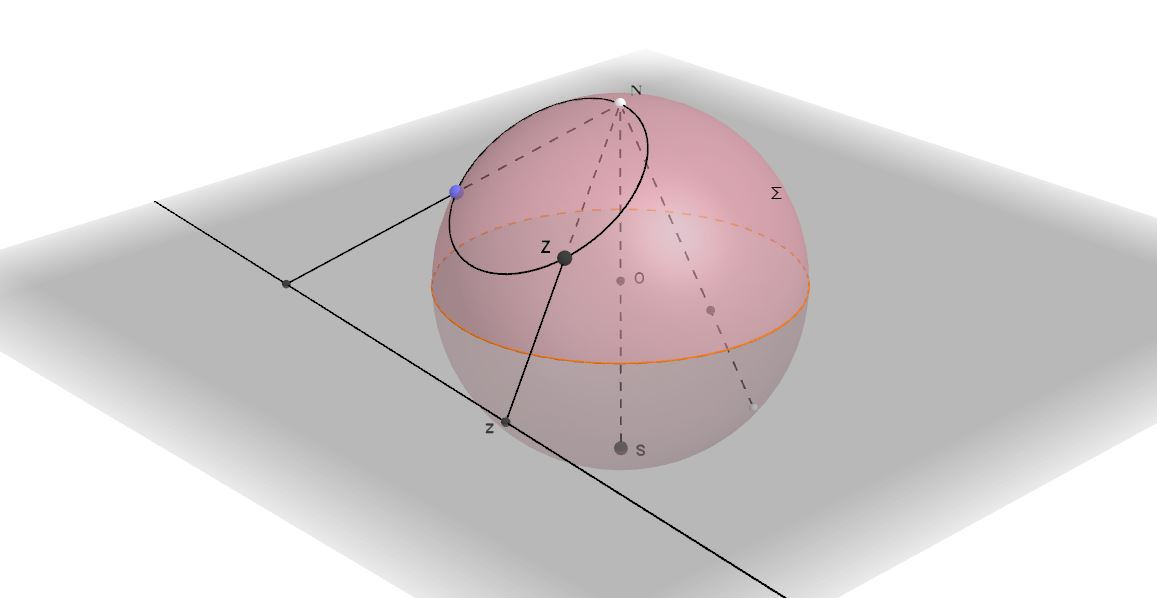
\includegraphics[scale=0.3]{stereo_proj.png}
L'inversion par rapport au cercle unité centré en $z=0$ est l'application $1/\overline{z}$ qui est une bijection du plan complexe privé de l'origine ; il en est de même de l'application $1/z$. Le point $0$ n'a pas d'image et réciproquement n'est l'image d'aucun point du plan. Pour remédier à cette difficulté, notons que lorsque le point $z$ s'approche de l'origine, son image $\omega=1/z$ s'éloigne de l'origine d'une distance de plus en plus grande dans n'importe quelle direction. Il serait donc intéressant d'adjoindre à $\C$ un point infini $\infty$ tel que 
\[\frac{1}{\infty}=0, \qquad \frac{1}{0}=\infty,\]
et tel que la fonction $1/z$ devienne une application bijective continue sur $\overline{\C}:= \C \cup \{\infty\}$. Pour conserver la continuité, il faut définir une topologie qui permette d'affirmer que lorsque $z$ tends vers $0$ alors $1/z$ tende vers $\infty$. La base des voisinages ouverts de $\C$ est l'ensemble des boules ouvertes d'où la définition suivante de la limite d'une fonction :
\begin{fdefn}
Soit $z_0, L\in \C$. La fonction $f$ a pour limite $L$ au point $z_0$ si : 
\[\forall \epsilon >0, \exists \delta >0, \;  \lvert z-z_0 \rvert < \delta \implies \lvert f(z)-L \rvert < \epsilon.\]
La fonction $f$ est continue en $z_0$ si $L=f(z_0)$.
\end{fdefn}

Pour étendre la topologie à $\overline{\C}$, de façon à rendre continue en $0$ la fonction $1/z$, un sous-ensemble $V$ sera un voisinage ouvert $V$ de $\infty$ si l'image réciproque de $V$ par l'application $1/z$ est un voisinage ouvert de $0$. En particulier, une base de voisinages de $\infty$ sera les ensembles
\[ B(\infty, r)=\{z  \in \overline{\C} : |z]>r\}, \quad r>0.\]
Une autre façon de dire cela consiste à définir les ouverts de l'infini comme les complémentaires dans $\overline{\C}$ des compacts de $\C$. Ceci permet d'étendre la définition d'une limite au point $z_0 = \infty$ par

\begin{fdefn}
On dira que la fonction $f : \C \mapsto \C$ a pour limite $L$ à l'infini si : 
\[\forall \epsilon >0, \exists \delta >0, \;  \lvert z \rvert > \delta \implies \lvert f(z)-L \rvert < \epsilon.\]
\end{fdefn}
Si $f$ admet une limite $L$ à l'infini, on peut la prolonger par continuité en posant $f(\infty)=L$. Une autre définition possible d'une limite à l'infini consiste à utiliser la transformation $1/z$ :

\begin{prop}
Soit $L \in \C$. Alors $\lim_{z \rightarrow \infty} f(z)= L$ si et seulement si $\lim_{z \rightarrow 0} f(1/z)= L$. De même $\lim_{z \rightarrow z_0} f(z)= \infty$ si et seulement si $\lim_{z \rightarrow z_0} 1/f(z)= 0$.
\end{prop}







Le fait d'adjoindre à $\C$ un point à l'infini permet d'obtenir un espace  $\overline{\C}$ compact isomorphe à la sphère de $\R^3$. Le moyen de se convaincre de se résultat est de considérer la projection stéréographique du plan complexe sur la sphère unité.  

\begin{figure}
\label{fig:sphereRiemann}
\begin{center}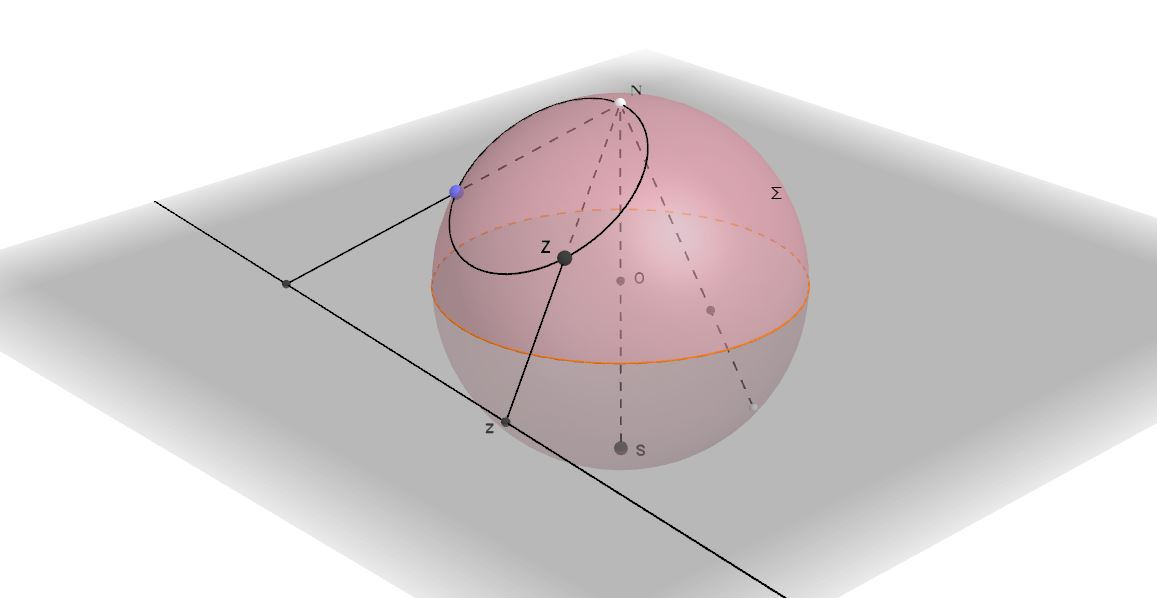
\includegraphics[scale=0.5]{stereo_proj}
\end{center}
\caption{Sphère de Riemann}
\end{figure}

Considérons dans $\R^3$, la sphère $\Sigma$ de rayon l'unité et centrée en l'origine (cf. figure~\ref{fig:sphereRiemann}). On projette le point d'affixe $z \in \C$ sur la sphère en considérant l'intersection $Z$ de la droite reliant $z$ au point $N=(0,0,1)$, appelé pôle Nord, avec la sphère $\Sigma$. Réciproquement un point $Z$ de la sphère est transformé en le point $z$, intersection de la droite passant par le pôle Nord et le point $Z$ avec le plan $\C$. Nous observons que le point $S=(0,0,-1)$, appelé pôle Sud est transformé en l'origine $O$ et que les points du cercle unité dans $\C$ sont invariant. De plus, l'image de toute calotte sphérique centrée en $N$ est un voisinage du point à l'infini. Il est donc naturel de considérer le pôle Nord comme le point à l'infini, et la transformation décrite est une bijection entre $\overline{\C}$ et la sphère $\Sigma$. Cette transformation est appelée projection stéréographique et la sphère $\Sigma$ est appelée sphère de Riemann. 

La transformation stéréographique associe à tout point $\hat{Z}=(X,Y,Z)$ de la sphère, lorsque $Z \neq 1$, le point $z=\frac{X+i Y}{1-Z}$, où bien si $\hat{Z} = (\phi,  \theta)$ (en coordonnées sphériques), le point $z= \cot (\phi/2) e^{i \theta}$.   





\subsection{Transformations de Möbius}

Nous avons caractérisé les similitudes qui sont des transformations bijectives du plan qui préservent les triangles. Puis, nous avons considéré l'inversion géométrique qui est une transformation bijective sur le plan privé d'un point, ce qui nous a conduit à compléter le plan complexe par un point à l'infini pour étendre cette application en une bijection sur $\bar{\C}$. Nous allons maintenant généraliser l'inversion en une classe de transformations bijectives sur $\bar{\C}$ (ou encore sur la sphère de Riemann) qui possèdent de très belles propriétés.

Une \textit{transformation de Möbius} ou \textit{homographie} est une application de la forme 
\[M(z)=\frac{a z +b}{c z +d},\]
où $a,b,c,d$ sont des constantes complexes. 

Notons tout d'abord que si $(ad-bc)=0$, l'application est une application constante qui envoie tous les points $z$ sur la même image $(a/c)$. Nous supposerons toujours dans la suite que $(ad-bc) \neq 0$. D'autre part $M(\infty)=a/c$ et $M(-d/c)=\infty$.

\begin{prop}
Une transformation de Möbius se décompose en la composition d'une suite de transformations :
\begin{MYenumerate}
\item $z \mapsto z +\frac{d}{c}$, qui est une translation ;
\item $z \mapsto \frac{1}{z}$ ;
\item $z \mapsto -\frac{(ad-bc)}{c^2}z$, qui est une rotation-homothétie ;
\item $z \mapsto z +\frac{a}{c}$, qui est une autre translation.
\end{MYenumerate}
\end{prop}

Chacune des transformations précédentes préservent les cercles, les angles et les symétries ; nous en déduisons directement les propriétés suivantes :
\begin{itemize}
\item Les transformations de Möbius transforment les cercles en cercles.
\item Les transformations de Möbius sont conformes.
\item Si deux points sont symétriques par rapport à un cercle, leurs images seront symétriques par rapport au cercle image.
\end{itemize}
Pour spécifier une transformation de Möbius particulière, il semble a priori nécessaire de déterminer les quatres nombres complexes,$a,b,c,d$. Cependant, pour tout complexe non nul $k$ 
\[M(z)= \frac{a z +b}{c z +d}=\frac{k a z +k b}{k c z +k d},\]
seuls les rapports entre les coefficients est important. Il est par exemple possible de choisir $k=\pm \sqrt{ad-bc}$, ce qui permet de se ramener à des coefficients satisfaisant la condition $ad-bc=1$. En fait, 

\emph{Il existe une unique transformation de Möbius envoyant trois points quelconques sur trois autres points quelconques.}

Une autre propriété importante est que l'ensemble des transformations de Möbius telle que $(ad-bc) \neq 0$ est un groupe pour la loi de composition. En particulier 
\[M^{-1}(z)=\frac{dz-b}{-cz +a}\]
et si 
\[M_1(z)=\frac{a_1 z +b_1}{c_1 z +d_1}, \quad M_2(z)=\frac{a_2 z +2}{c_2 z +d_2},\]
alors
\[(M_2 \circ M_1)(z)=\frac{(a_2 a_1 + b_2 c_1) z + (a_2 b_1 + b_2 d_1)}{(c_2a_1 + d_2 c_1)z +(c_2 b_1 + d_2 d_1)}.\]
Une façon assez simple de trouver ces formules consiste à représenter la transformation $M(z)$ par la matrice
\[M(z)=\frac{a z +b}{cz +d} \longleftrightarrow M=\begin{pmatrix}
a &b\\c&d
\end{pmatrix},\]
et donc la matrice associée à l'inverse de $M(z)$ est la transformation associée à la matrice $M^{-1}$ qui existe en raison de l'hypothèse $(ad -bc) \neq 0$ qui traduit que $\det(M) \neq 0$. De plus la matrice associée à $(M_2 \circ M_1)(z)$ est la transformation de associée à la matrice $M_2 M_1$. 


Les points fixes d'une transformation de Möbius $M(z)$ sont les solutions de l'équation 
\[z=M(z)=\frac{a z +b}{c z +d}.\]
Celle-ci étant quadratique, nous en déduisons qu'à l'exception de l'identité, une transformation de Möbius possède au plus deux points fixes. Il s'ensuit que si une transformation de Möbius présente plus de deux points fixes, elle est nécessairement l'identité. Supposons donc que $M$ et $N$ sont deux transformations de Möbius envoyant trois points donnés ($p,q,r$ par ex.) sur trois points images, alors pour la transformation de Möbius $N^{-1} \circ M$ ces trois points sont fixes et donc $N=M$. Ceci implique l'unicité de la transformation dont les images de trois points donnés sont fixées. Par exemple, la transformation envoyant les points $p,q,r$ sur $0,1,\infty$ est la transformation, notée $[z,p,q,r]$, suivante :
\[[z,p,q,r] =\frac{(z-p)(q-r)}{(z-r)(q-p)},\]
expression connue sous le nom de birapport ou de rapport anharmonique.

Pour trouver l'expression d'une transformation de Möbius $M(z)$ transformant les points $(p,q,r)$ en $(p',q',r')$ respectivement, il suffit de considérer les deux transformations $M_1$ et $M_2$ transformant respectivement $(p,q,r)$ et $(p',q',r')$ en $(0,1,\infty)$, car $M(z)=(M_2^{-1} \circ M_1)(z)$. Donc, en posant $\omega =M(z)$, il découle de la décomposition précédente l'identité $M_2(\omega)=M_1(z)$ soit :
\begin{equation}\label{eq:Mob1}\frac{(\omega-p')(q'-r')}{(\omega-r')(q'-p')} = [\omega,p',q',r']=[z,p,q,r]=\frac{(z-p)(q-r)}{(z-r)(q-p)}.
\end{equation}

Cette relation peut s'interpréter de la façon suivante : les points $a,p,q,r$ ont pour images respectives les points $a',p',q',r'$ par une transformation de Möbius si et seulement si leurs birapport sont égaux. Par conséquent, soit $C$ l'unique cercle passant par les points $p,q,r$, dont le bord est orienté de façon à parcourir les points dans l'ordre mentionné. La transformation de Möbius donnée par~(\ref{eq:Mob1}) transforme le cercle $C$ sur le cercle $C'$ orienté passant par les points $p',q',r'$ de telle façon que la région à gauche de $C$ (en se déplaçant selon l'orientation du cercle) est envoyée sur la région à gauche de $C'$ (cf. figure~(\ref{fig:Mob2})).


\begin{figure}[ht]
\begin{center}
\begin{tikzpicture}[line cap=round,line join=round,>=triangle 45,x=1.0cm,y=1.0cm, scale=0.6]
\draw[fill=white](-5,-5) rectangle (5,5);
\fill [color=gray] (0.,0.) circle (3.cm);
\draw[color=black, decoration={markings, mark=at position 0.3 with {\arrow{>}}, mark=at position 0.625 with {\arrow{>}}, mark=at position 0.95 with {\arrow{>}}},
        postaction={decorate}] (0.,0.) circle (3.cm);
\draw (-2.1702,-0.9978) node[anchor=north west] {$C$};
\draw (2.694,2.5112) node[anchor=north west] {$p$};
\draw (-3.1382,2.0756) node[anchor=north west] {$q$};
\draw (1.3146,-2.7402) node[anchor=north west] {$r$};
\begin{scriptsize}
\draw [color=black,fill=white] (2.301408120092678,1.9244533418016363) circle (2.5pt);
\draw [color=black,fill=white] (-2.5898903823572463,1.514089761993468) circle (2.5pt);
\draw [color=black,fill=white] (1.3255494676471464,-2.691267100980571) circle (2.5pt);
\end{scriptsize}

\begin{scope}[xshift=12cm]
\fill[color=gray] (-5,-5) rectangle (5,5);
\fill [color=white, opacity=1] (0.,0.) circle (3.cm);
\draw[color=black, decoration={markings, mark=at position 0.3 with {\arrow{<}}, mark=at position 0.625 with {\arrow{<}}, mark=at position 0.9 with {\arrow{<}}},
        postaction={decorate}] (0.,0.) circle (3.cm);
\draw (-2.1702,-0.9978) node[anchor=north west] {$C'$};
\draw (3.0812,-0.3202) node[anchor=north west] {$p'$};
\draw (1.2904,-2.7402) node[anchor=north west] {$q'$};
\draw (-3.6222,0.672) node[anchor=north west] {$r'$};
\begin{scriptsize}
\draw [color=black, fill=white] (2.961048665728481,-0.4818618050723474) circle (2.5pt);
\draw [color=black,fill=white] (1.2823751372933847,-2.7121050877965205) circle (2.5pt);
\draw [color=black,fill=white] (-2.996381114672065,0.14730993054303543) circle (2.5pt);
\end{scriptsize}
\end{scope}
\end{tikzpicture}
\caption{Image d'un cercle passant par trois points par une transformation de Möbius} \label{fig:Mob2}
\end{center}
\end{figure}

En particulier, la transformation de Möbius $[z,p,q,r]$ transporte le cercle passant par $p,q,r$ sur l'axe réel de telle façon que ces trois points soient envoyés sur $0,1,\infty$. Avec l'orientation positive induite par l'ordre de ces points l'intérieur du cercle est envoyé sur le demi-plan supérieur ($\text{Im} z \geq 0$) (cf. figure~\ref{fig:Mob3}) 

\begin{figure}[ht] 
\begin{center}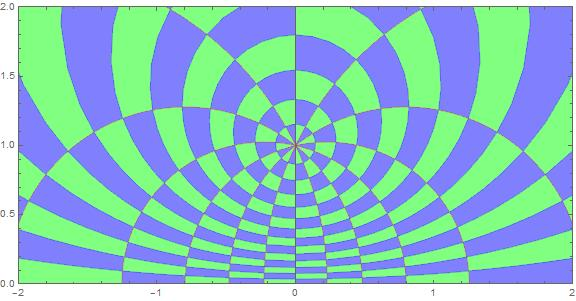
\includegraphics[scale=0.5]{mobius_disk_plan}
\end{center}
\caption{Image du disque unité par $M(z)=[z,-1,i,1] = i \frac{1+z}{1-z}$}\label{fig:Mob3}
\end{figure}

\section{Exercices complémentaires}


\begin{exer}[cf. \cite{needham1998visual}] \label{exer:I0} Montrer que l'aire du parallélogramme de sommets $a,b,c,d$ (énoncé dans le sens contraire des aiguilles d'une montre) est donnée par
$$\frac{1}{2}\text{Im} \left[\overline{a} b + \overline{b}c + \overline{c}d + \overline{d}a\right].$$
Indication : décomposer le parallélogramme en quatre triangles et faire attention aux signes des aires de chaque triangle en fonction de la position de l'origine à l'intérieur ou l'extérieur du parallélogramme.
\begin{figure}[ht]
\begin{center}
\shorthandoff{!}\shorthandoff{:}
\begin{tikzpicture}[line cap=round,line join=round,>=triangle 45,x=1.0cm,y=1.0cm, scale=0.5]
%\clip(-4.3,-5.28) rectangle (23.02,6.3);
\fill[color=gray!30,fill=gray!30,fill opacity=0.1] (-1.38,3.16) -- (0,0) -- (2.56,1.4) -- cycle;
\fill[color=gray!30,fill=gray!30,fill opacity=0.1] (0,0) -- (-2.68,-2.06) -- (2,-3.14) -- cycle;
\fill[fill=black,pattern=north east lines] (0,0) -- (2.56,1.4) -- (2,-3.14) -- cycle;
\fill[color=gray!30,fill=gray!30,fill opacity=0.15] (7,0) -- (9.78,3.14) -- (13.72,1.38) -- cycle;
\fill[color=gray!30,fill=gray!30,fill opacity=0.2] (7,0) -- (13.16,-3.16) -- (8.48,-2.08) -- cycle;
\fill[fill=black,pattern=north east lines] (7,0) -- (9.78,3.14) -- (8.48,-2.08) -- cycle;
\draw (2.56,1.4)-- (-1.38,3.16);
\draw (-1.38,3.16)-- (-2.68,-2.06);
\draw (-2.68,-2.06)-- (2,-3.14);
\draw (2,-3.14)-- (2.56,1.4);
\draw [color=gray!30] (-1.38,3.16)-- (0,0);
\draw [color=gray!30] (0,0)-- (2.56,1.4);
\draw [color=gray!30] (2.56,1.4)-- (-1.38,3.16);
\draw [color=gray!30] (0,0)-- (-2.68,-2.06);
\draw [color=gray!30] (-2.68,-2.06)-- (2,-3.14);
\draw [color=gray!30] (2,-3.14)-- (0,0);
\draw (0,0)-- (2.56,1.4);
\draw (2.56,1.4)-- (2,-3.14);
\draw (2,-3.14)-- (0,0);
\draw (0,0)-- (-1.38,3.16);
\draw (-1.38,3.16)-- (-2.68,-2.06);
\draw (-2.68,-2.06)-- (0,0);
\draw (13.72,1.38)-- (9.78,3.14);
\draw (9.78,3.14)-- (8.48,-2.08);
\draw (8.48,-2.08)-- (13.16,-3.16);
\draw (13.16,-3.16)-- (13.72,1.38);
\draw [color=gray!30] (7,0)-- (9.78,3.14);
\draw [color=gray!30] (9.78,3.14)-- (13.72,1.38);
\draw [color=gray!30] (13.72,1.38)-- (7,0);
\draw [color=gray!30] (7,0)-- (13.16,-3.16);
\draw [color=gray!30] (13.16,-3.16)-- (8.48,-2.08);
\draw [color=gray!30] (8.48,-2.08)-- (7,0);
\draw (7,0)-- (9.78,3.14);
\draw (9.78,3.14)-- (8.48,-2.08);
\draw (8.48,-2.08)-- (7,0);
\begin{scriptsize}
\fill [color=pblue] (2.56,1.4) circle (1.5pt);
\draw[color=pblue] (2.7,1.68) node {$A$};
\fill [color=pblue] (-1.38,3.16) circle (1.5pt);
\draw[color=pblue] (-1.58,3.4) node {$B$};
\fill [color=pblue] (-2.68,-2.06) circle (1.5pt);
\draw[color=pblue] (-2.94,-1.94) node {$C$};
\fill [color=pblue] (2,-3.14) circle (1.5pt);
\draw[color=pblue] (2.24,-3.28) node {$D$};
\fill [color=pblue] (0,0) circle (1.5pt);
\draw[color=pblue] (-0.36,0.28) node {$O$};
\fill [color=pblue] (13.72,1.38) circle (1.5pt);
\draw[color=pblue] (13.86,1.66) node {A};
\fill [color=pblue] (9.78,3.14) circle (1.5pt);
\draw[color=pblue] (9.58,3.38) node {B};
\fill [color=pblue] (8.48,-2.08) circle (1.5pt);
\draw[color=pblue] (8.22,-1.96) node {C};
\fill [color=pblue] (13.16,-3.16) circle (1.5pt);
\draw[color=pblue] (13.4,-3.3) node {D};
\fill [color=pblue] (7,0) circle (1.5pt);
\draw[color=pblue] (6.9,0.26) node {O};
\end{scriptsize}
\end{tikzpicture}
\shorthandon{!}\shorthandoff{:}
\caption{}\label{fig:exer}
\end{center}
\end{figure}
\end{exer}


\begin{exer}\label{exer:I1} Le but de cet exercice est de montrer que l'ensemble des points $M$ vérifiant la condition $MA/MB=k$ ($k \neq 1$) est un cercle, appelé cercle d'Apollonius. Bien que ce résultat puisse se prouver par des arguments classiques de géométrie euclidienne, nous utiliserons les nombres complexes. 
\begin{MYenumerate}
\item Soient $p$ et $q$ les affixes respectives des points $A$ et $B$, montrer que l'équation
$$\left| \frac{z-p}{z-q}\right|=k, \quad k\neq 1$$
définit un cercle de centre $z_0$ et de rayon $\rho$ (donc $z$ est solution de l'équation $|z-z_0|=\rho$) à déterminer. 
\item Montrer que $|p-z_0||q-z_0|= \rho^2$~: nous verrons ultérieurement que ceci signifie que les points $A$ et $B$ sont liés par l'inversion de pôle le point d'affixe $z_0$ et de puissance $\rho^2$.
\item Que peut-on dire lorsque $k=1$~?
\end{MYenumerate}
\end{exer}

\begin{exer}\label{exer:I2}
\begin{MYenumerate}
\item Montrer qu'une transformation $z'=az+b$ est une translation si $a=1$, sinon une similitude directe de rapport $k=|a|$, d'angle $\theta=\arg(a)$ et de centre le point $I$ d'affixe $b/(1-a)$. 
\item Pour prouver que toute similitude directe est de la forme $z'=az+b$, considérer les points $O, A$ d'affixes respectives $0$ et $1$. Soient $O'$, $A'$ les images (distinctes) de $O$ et $A$ par cette transformation et $b$ et $c$ leurs affixes. Soient $M \neq O$ un point quelconque d'affixe $z$ et son image $M'$ d'affixe $z'$. Déduire des conditions suivantes~:
$$\frac{O'M'}{O'A'}=\frac{OM}{OA} \quad \text{ et } \quad  (A',O',M')=(A,O,M)$$
la forme voulue de la transformation.                      
\end{MYenumerate}
\end{exer}


\begin{exer} Montrer que 
\begin{MYenumerate}
\item toute similitude plane qui fixe trois points distincts non alignés est l'identité,
\item toute similitude plane qui fixe deux points $A$ et $B$ distincts est soit l'identité soit une réflexion d'axe la droite (AB).
\end{MYenumerate}
\textbf{Indication} : Utiliser soit une approche géométrique en montrant tout d'abord que la similitude est nécessaire une isométrie et en faisant apparaître une médiatrice, soit en utilisant l'approche algébrique.
\end{exer}


\begin{exer}\label{exer:I3} Soient deux points distincts $A$ et $B$ et $A'\neq A$ et $B'\neq B$ leurs images respectives par inversion. Pour démontrer que les points $A,A', B,B'$ sont cocycliques, rappelons tout d'abord la définition classique de la puissance d'un point par rapport à un cercle.

\emph{Soit $C$ un cercle de centre $O$ et de rayon $R$, $A$ un point du plan et
$D$ une droite passant par $A$ et coupant $C$ en deux points $B$ et $C$. Alors le produit scalaire $\stackrel{\longrightarrow}{AB} \cdot \stackrel{\longrightarrow}{AC}$ est égal à $AO^2-R^2$ et ne dépend donc pas de la droite $D$. Ce nombre est appelé puissance de $A$ par rapport au cercle $C$ et noté $p_C(A)$.} 

La puissance permet de situer $A$ par rapport au cercle, car $A$ est à l'extérieur du cercle, sur le cercle ou à l'intérieur du cercle si et seulement si $p_C(A)$ est respectivement positif, nul ou négatif. En particulier, si $A$ est extérieur au cercle $C$, alors $p_C(A) = AT^2=AT'^2$, où $T$ et $T'$ sont les points de contact des deux tangentes menées par $A$ au cercle $C$.
 

\begin{figure}[ht]
\begin{center}
\shorthandoff{!}\shorthandoff{:}
\begin{tikzpicture}[line cap=round,line join=round,>=triangle 45,x=1.0cm,y=1.0cm]
%\clip(-4.3,-7.76) rectangle (24.16,6.3);
\clip(-4.3,-2.16) rectangle (11.02,3.3);
\draw(4.98,0.02) circle (2cm);
\draw [color=pred] (3.37,1.21)-- (5.75,-1.83);
\draw [color=pred] (6.03,1.72)-- (3.55,-1.37);
\draw [color=pgreen] (4.47,1.95)-- (3.37,1.21);
\draw [color=pgreen] (4.47,1.95)-- (6.03,1.72);
\draw (-3.02,-0.02)-- (4.47,1.95);
\draw (-3.02,-0.02)-- (5.75,-1.83);
\draw (-3.02,-0.02)-- (6.03,1.72);
\begin{scriptsize}
\fill [color=pblue] (4.98,0.02) circle (1.5pt);
\draw[color=pblue] (5.14,0.3) node {$O$};
\fill [color=pblue] (-3.02,-0.02) circle (1.5pt);
\draw[color=pblue] (-2.88,0.26) node {$A$};
\fill [color=pblue] (3.37,1.21) circle (1.5pt);
\draw[color=pblue] (3.54,1.5) node {$B$};
\fill [color=pblue] (3.55,-1.37) circle (1.5pt);
\draw[color=pblue] (3.7,-1.1) node {$D$};
\fill [color=pblue] (6.03,1.72) circle (1.5pt);
\draw[color=pblue] (6.2,2) node {$C$};
\fill [color=pblue] (5.75,-1.83) circle (1.5pt);
\draw[color=pblue] (5.9,-1.54) node {$E$};
\fill [color=pblue] (4.47,1.95) circle (1.5pt);
\draw[color=pblue] (4.62,2.24) node {$T$};
\end{scriptsize}
\end{tikzpicture}
\shorthandon{!}\shorthandoff{:}
\caption{Puissance du point $A$ par rapport au cercle $C$ de centre $O$.}\label{fig2}
\end{center}
\end{figure}
Réciproquement, si deux droites $(BC)$, $(DE)$ se coupent en un point $A$ de telle façon que $AB \cdot AC= AD \cdot AE$ (dans l'ordre), alors les points $B,C,D,E$ sont cocycliques. 

Utiliser ce résultat pour vérifier que, pour une inversion, les points $A,A',B,B'$ sont cocycliques ou alignés.

\end{exer}

\begin{exer}[\cite{needham1998visual}] L'utilisation de l'inversion permet de prouver des résultats géométriques portant sur les cercles de façon élégante. Par exemple, considérons le théorème de Ptolémée qui affirme que pour quatre points distincts cocycliques $A,B,C,D$, formant ainsi un quadrilatère (cf. figure~\ref{fig7}), alors la somme des produits des longueurs des côtés opposés est égale au produit des longueurs des diagonales~:
$$AD \cdot BC + AB \cdot CD=AC\cdot BD.$$
\begin{figure}[ht]
\begin{center}
\shorthandoff{!}\shorthandoff{:}
\begin{tikzpicture}[line cap=round,line join=round,>=triangle 45,x=1.0cm,y=1.0cm, scale=0.5]
%\clip(-12.55,-12.95) rectangle (36.93,7.68);
\clip(-12.55,-7) rectangle (15,8);

\draw(2.99,0.57) circle (3.23cm);
\draw (2.28,3.72)-- (0.38,-1.34);
\draw (0.38,-1.34)-- (3.18,-2.66);
\draw (3.18,-2.66)-- (6.13,1.32);
\draw (6.13,1.32)-- (2.28,3.72);
\draw [dash pattern=on 5pt off 5pt] (0.38,-1.34)-- (6.13,1.32);
\draw [dash pattern=on 5pt off 5pt] (2.28,3.72)-- (3.18,-2.66);
\draw [dotted] (2.28,3.72) circle (7.59cm);
\draw [domain=-12.55:36.93] plot(\x,{(-85.92--3.27*\x)/14.51});
\draw [dotted] (0.38,-1.34)-- (-1.46,-6.25);
\draw [dotted] (3.18,-2.66)-- (3.53,-5.13);
\draw [dotted] (6.13,1.32)-- (13.04,-2.99);
\begin{scriptsize}
\fill [color=pblue] (2.28,3.72) circle (2.0pt);
\draw[color=pblue] (2.41,4.38) node {$A$};
\fill [color=pblue] (0.38,-1.34) circle (2.0pt);
\draw[color=pblue] (-0.16,-1.19) node {$B$};
\fill [color=pblue] (3.18,-2.66) circle (2.0pt);
\draw[color=pblue] (3.62,-2.8) node {$C$};
\fill [color=pblue] (6.13,1.32) circle (2.0pt);
\draw[color=pblue] (6.58,1.78) node {$D$};
\draw[color=black] (-3,-2) node {K};
\fill [color=pblue] (-1.46,-6.25) circle (2.0pt);
\draw[color=pblue] (-1.15,-5.66) node {$B'$};
\fill [color=pblue] (3.53,-5.13) circle (2.0pt);
\draw[color=pblue] (3.87,-4.56) node {$C'$};
\fill [color=pblue] (13.04,-2.99) circle (2.0pt);
\draw[color=pblue] (13.36,-2.4) node {$D'$};
\end{scriptsize}
\end{tikzpicture}
\shorthandon{!}\shorthandoff{:}
\caption{Théorème de Ptolémée }\label{fig7}
\end{center}
\end{figure}

Considérer une inversion de cercle $K$ centré en un des quatre points, $A$ par exemple, et de rayon $R$ suffisamment grand pour englober en son intérieur le cercle circonscrit au quadrilatère, et montrer que les images $B'$, $C'$ et $D'$ des points $B,C,D$ sont alignés. En déduire une relation liant les longueurs $B'C'$, $C'D'$ et $B'D'$. Maintenant, en utilisant la propriété sur les triangles semblables ($BAC$ est semblable à $C'AB'$) établir une relation entre les longueurs $BC$ et $B'C'$, puis conclure.
\end{exer}


\begin{exer}[\textbf{Projection stéréographique}]
Le but de cet exercice est d'établir une formule explicite connectant le point $z = x +i y \in \C$ et sa projection $\hat{z}$ sur $\Sigma$. Soit $(X,Y,Z)$ les coordonnées cartésiennes de $\hat{z}$, où l'axe $Z$ passe par $N$ et les axes $X$ et $Y$ coïncident avec les axes $x,y$ de $\C$.  Soit $z' = X+i Y$ le pied de la perpendiculaire à $\C$ passant par $\hat{z}$. 

\begin{figure}[ht]
\begin{center}
\shorthandoff{!}\shorthandoff{:}
\begin{tikzpicture}[line cap=round,line join=round,>=triangle 45,x=9.999999999999998cm,y=10.0cm, scale=0.3]
\clip(-1.0204444716563346,-1.1991274885913612) rectangle (2.500817665540407,1.2986943169702587);
\draw[fill opacity=0.10000000149011612] (0.055454528631341884,0.6249841873023777) -- (0.05545452863134189,0.6804387159337196) -- (0.,0.6804387159337196) -- (0.,0.6249841873023777) -- cycle; 
\draw[fill opacity=0.10000000149011612] (0.055454528631341884,0.) -- (0.05545452863134189,0.05545452863134188) -- (0.,0.055454528631341884) -- (0.,0.) -- cycle; 
\draw[fill opacity=0.10000000149011612] (0.8360919384587128,0.) -- (0.8360919384587128,0.05545452863134188) -- (0.7806374098273708,0.055454528631341884) -- (0.7806374098273708,0.) -- cycle; 
\draw(0.,0.) circle (10.cm);
\draw (0.,1.)-- (2.081611983804011,0.);
\draw (0.,0.)-- (0.7806374098273708,0.6249841873023777);
\draw (0.5519676853769542,-0.8697443933524662) node[anchor=north west] {$\Sigma$};
\draw (-0.09895605045228752,-0.010995609336775847) node[anchor=north west] {$O$};
\draw (-0.11464095974937767,1.1849787245663546) node[anchor=north west] {$N$};
\draw (0.8225323707517594,0.7850135374905536) node[anchor=north west] {$\hat{z}$};
\draw (2.0930100238160625,0.13016857433703627) node[anchor=north west] {$z$};
\draw [line width=0.4pt] (0.,0.6249841873023777)-- (0.7806374098273708,0.6249841873023777);
\draw [line width=0.4pt] (0.7806374098273708,0.6249841873023777)-- (0.7806374098273708,0.);
\draw (0.7558715062391264,-0.003153154688230729) node[anchor=north west] {$z'$};
\draw (0.573525732429403,0.38112712309048) node[anchor=north west] {$Z$};
\draw (-0.14993200566783055,0.5732672619798354) node[anchor=north west] {$1$};
\draw [domain=-1.0204444716563346:2.500817665540407] plot(\x,{(-0.-0.*\x)/-2.081611983804011});
\draw (0.,1.)-- (0.,0.);
\begin{scriptsize}
\fill [color=pblue] (0.,0.) circle (5pt);
\fill [color=pblue] (0.,1.) circle (5pt);
\fill [color=pblue] (0.7806374098273708,0.6249841873023777) circle (5pt);
\fill [color=pblue] (2.081611983804011,0.) circle (5pt);
\fill [fill=pblue] (0.,0.6249841873023777) circle (5pt);
\fill [color=pblue] (0.7806374098273708,0.) circle (5pt);
\end{scriptsize}
\end{tikzpicture}

\shorthandon{!}\shorthandoff{:}
\caption{Projection stéréographique}\label{fig8}
\end{center}
\end{figure}

Alors $z'$ et $z$ sont dans la même direction, ainsi
\[z=\frac{\lvert z \rvert}{\lvert z' \rvert} z'.\]
\begin{MYenumerate}
\item En observant la figure~\ref{fig8}, qui représente la section verticale de la sphère et de $\C$ passant par $N$ et $\hat{z}$, que les triangles rectangles d'hypoténuse $N \hat{z}$ et $Nz$ sont semblables, en déduire que 
\[\frac{\lvert z \rvert}{\lvert z' \rvert} = \frac{1}{1-Z}.\]
\item Obtenir la première formule
\[x+iy = \frac{X+i Y}{1-Z},\]
puis l'inverser pour trouver les coordonnées de $\hat{z}$ en fonction des coordonnées de $z$.
\item Une cercle sur $\Sigma$ passant par le point $N=(0,0,1)$ est l'intersection du plan d'équation $a X + b Y +c(Z-1)=0$ avec $\Sigma$. En déduire que les images $z$ vérifient une équation de la forme
\[\bar{\omega} z + \omega \bar{z}=k \]
avec $\omega  \in \C^\ast$ et $k \in \R$ que l'on exprimera en fonction des constantes réelles $a,b,c$. Montrer que l'on obtient l'équation d'une droite dans $\C$.
\item Si le cercle ne passe pas par $N$, en raison de la symétrie de la sphère, une simple rotation permet de considérer le cercle comme l'intersection du plan $Z=k$ avec $\Sigma$ (avec $k>0$). Montrer alors que $\lvert z\rvert ^2$ est constant et donc que l'image est un cercle centré à l'origine.  
\end{MYenumerate}
Il existe des démonstration purement géométrique de ces résultats, par exemple dans l'excellent livre \cite{hilbert1983geometry}.
\end{exer}